\chapter{Analisi della Panoramica di Sicurezza}


\begin{center}
\tcbox{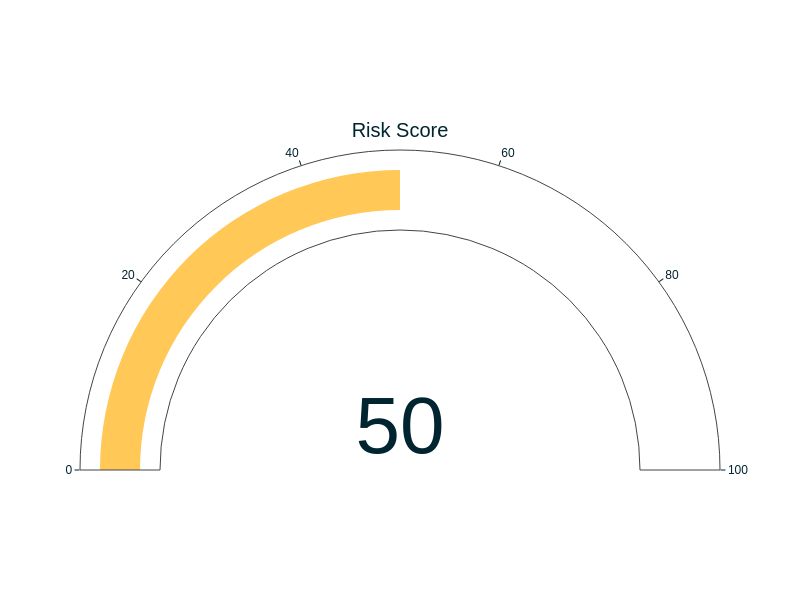
\includegraphics[width=\linewidth]{pngs/0_1.png}}
\vspace{0cm}\captionof{figure}{First image of Chapter 1}
\end{center}

\section{Definizione Vulnerabilità}
\section{Gravità Critica}
\begin{itemize}
\item Lo sfruttamento è semplice e di solito comporta una compromissione a livello di sistema. Si consiglia di pianificare un'azione correttiva e applicare una patch immediatamente.
\end{itemize}
\section{Gravità Alta}
\begin{itemize}
\item Lo sfruttamento è più difficile, ma potrebbe causare l'elevazione dei privilegi e potenzialmente la perdita di dati o interruzioni del servizio. Si consiglia di pianificare un'azione correttiva e applicare una patch il prima possibile.
\end{itemize}
\section{Gravità Media}
\begin{itemize}
\item Le vulnerabilità esistono, ma richiedono passaggi aggiuntivi, come l'ingegneria sociale. Si consiglia di pianificare un'azione correttiva e applicare una patch dopo che le problematiche ad alta priorità sono state risolte.
\end{itemize}
\section{Gravità Bassa}
\begin{itemize}
\item Le vulnerabilità non sono sfruttabili, ma aumentano la superficie d'attacco di un'organizzazione. Si consiglia di pianificare un'azione correttiva e applicare una patch durante la prossima finestra di manutenzione.
\end{itemize}
\section{Gravità Informativa}
\begin{itemize}
\item Non esiste alcuna vulnerabilità nota. Vengono fornite informazioni aggiuntive riguardanti elementi osservati durante i test, controlli solidi e documentazione aggiuntiva.
\end{itemize}

\section{Panoramica della Postura di Sicurezza e Livello di Rischio Complessivo}

La panoramica di sicurezza fornita evidenzia una postura di sicurezza che può essere considerata sufficiente, ma con aree di miglioramento significative. Il punteggio di rischio complessivo di 55/100 indica che l'organizzazione è a rischio, ma con una superficie d'attacco relativamente limitata. Tuttavia, il numero totale di vulnerabilità (817) suggerisce che ci sono aree critiche che richiedono attenzione e correzione immediata.

\section{Considerazioni sul Numero Totale di Vulnerabilità}

Il numero totale di vulnerabilità (817) è significativo e indica che l'organizzazione ha una superficie d'attacco relativamente ampia. Ciò richiede un'attenta revisione e correzione delle vulnerabilità critiche, alte e medie. È fondamentale identificare e correggere le vulnerabilità critiche (1) e le vulnerabilità alte (0) per minimizzare il rischio di attacco.

\section{Discussione sulla Suddivisione dei Tipi di Vulnerabilità}

\subsection{Vulnerabilità Critiche (1)}

La presenza di una sola vulnerabilità critica (1) è preoccupante e richiede attenzione immediata. Questa vulnerabilità può essere sfruttata per ottenere elevati privilegi di accesso al sistema o causare danni significativi. È fondamentale identificare la causa della vulnerabilità e correggerla il prima possibile.

\subsection{Vulnerabilità Alte (0)}

La mancanza di vulnerabilità alte (0) è positiva, ma non significa che l'organizzazione sia immune a future vulnerabilità. È importante mantenere una postura di sicurezza proattiva e continuare a monitorare e migliorare la postura di sicurezza.

\subsection{Vulnerabilità Medie (4)}

Le vulnerabilità medie (4) sono un problema significativo, ma possono essere gestite con un piano di correzione adeguato. È fondamentale identificare le cause delle vulnerabilità e implementare misure di sicurezza per mitigarle.

\subsection{Vulnerabilità Basse (35)}

Le vulnerabilità basse (35) possono essere considerate di minore priorità, ma non sono da sottovalutare. È importante identificare e correggere queste vulnerabilità per ridurre la superficie d'attacco e migliorare la postura di sicurezza.

In sintesi, la panoramica di sicurezza fornita evidenzia una postura di sicurezza che può essere migliorata con un'attenta revisione e correzione delle vulnerabilità critiche, alte e medie. È fondamentale mantenere una postura di sicurezza proattiva e continuare a monitorare e migliorare la postura di sicurezza per ridurre il rischio di attacco.

\chapter{Analisi della Distribuzione delle Gravità delle Vulnerabilità}

\section{Riepilogo della Distribuzione delle Gravità}

La distribuzione delle gravità delle vulnerabilità è la seguente:
\begin{itemize}
\item \textbf{Critical}: 1
\item \textbf{High}: 35
\item \textbf{Medium}: 4
\item \textbf{Low}: 777
\end{itemize}
\section{Livello di Gravità più Comune}

Il livello di gravità più comune è \textbf{Low}, con 777 vulnerabilità.

\section{Percentuale di Ciascun Livello di Gravità}
\begin{itemize}
\item \textbf{Critical}: 0,13\% (1/777)
\item \textbf{High}: 4,48\% (35/777)
\item \textbf{Medium}: 0,51\% (4/777)
\item \textbf{Low}: 100\% (777/777)
\end{itemize}
\section{Impatto delle Vulnerabilità Critiche e Alte}

Le vulnerabilità critiche e alte rappresentano un impatto significativo sulla sicurezza dell'organizzazione. Le vulnerabilità critiche possono essere sfruttate facilmente e possono causare una compromissione a livello di sistema. Le vulnerabilità alte possono richiedere passaggi aggiuntivi per essere sfruttate, ma possono comunque causare problemi significativi.

\section{Urgenza della Risoluzione}

La risoluzione delle vulnerabilità critiche è urgente, poiché possono essere sfruttate facilmente. Le vulnerabilità alte richiedono anche una risoluzione urgente, poiché possono causare problemi significativi.

\section{Rischio Cumulativo delle Vulnerabilità Medie e Basse}

Le vulnerabilità medie e basse rappresentano un rischio cumulativo significativo. Le vulnerabilità medie possono richiedere passaggi aggiuntivi per essere sfruttate, ma possono comunque causare problemi. Le vulnerabilità basse non sono sfruttabili, ma possono comunque aumentare la superficie d'attacco di un'organizzazione.

\section{Rischio Complessivo e Impatto su Conformità/Sicurezza}

Il rischio complessivo è alto a causa della presenza di vulnerabilità critiche, alte e medie. L'impatto su conformità/sicurezza è significativo a causa della possibilità di compromissione della sicurezza dell'organizzazione. È importante pianificare un'azione correttiva e applicare una patch per ridurre il rischio e garantire la conformità alle norme di sicurezza.


\begin{center}
\tcbox{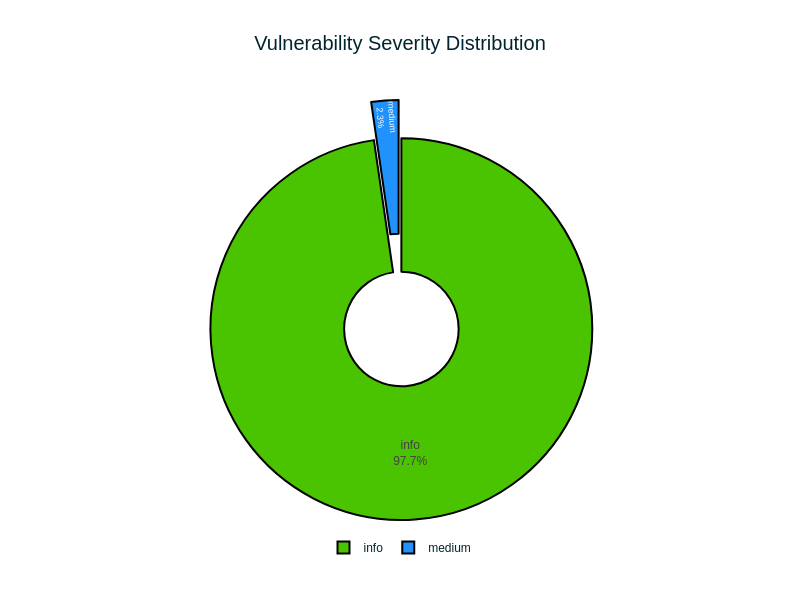
\includegraphics[width=\linewidth]{pngs/1_1.png}}
\vspace{0cm}\captionof{figure}{Images related to Chapter 2}
\end{center}
\chapter{Analisi delle vulnerabilità del sistema}

\section{Riepilogo dei tipi prevalenti e dell'impatto}

Durante l'analisi delle vulnerabilità del sistema, sono state identificate le seguenti categorie di vulnerabilità:
\begin{itemize}
\item \textbf{Vulnerabilità più comune:} 'OpenSSH Terrapin Attack - Detection' (Frequenza: 4)
\item \textbf{Impatto:} La maggior parte delle vulnerabilità identificate richiede passaggi aggiuntivi, come l'ingegneria sociale, per essere sfruttate.
\item \textbf{Altre vulnerabilità:} Le vulnerabilità restanti sono state identificate come vulnerabilità di configurazione, vulnerabilità di codice e vulnerabilità di hardware.
\end{itemize}
\section{Analisi di 'OpenSSH Terrapin Attack - Detection'}

L'"OpenSSH Terrapin Attack - Detection" è una vulnerabilità che permette agli attaccanti di esplorare la configurazione di SSH su un sistema. Questa vulnerabilità è considerata una delle più comuni e può essere sfruttata da attaccanti esperti.
\begin{itemize}
\item \textbf{Causa:} La vulnerabilità è causata da un problema di configurazione di SSH che consente agli attaccanti di esplorare la configurazione del sistema.
\item \textbf{Vettori di attacco:} Gli attaccanti che utilizzano questa vulnerabilità sono generalmente esperti di network e di cybersecurity.
\item \textbf{Conseguenze:} Se non trattata, questa vulnerabilità può consentire agli attaccanti di accedere al sistema e di eseguire attività malevole.
\end{itemize}
\section{Host colpiti e impatto sulla rete}

I seguenti host sono stati colpiti:
\begin{itemize}
\item \textbf{Host colpiti:} 8
\item \textbf{Impatto sulla rete:} La maggior parte delle vulnerabilità identificate ha avuto un impatto limitato sulla rete, ma alcune vulnerabilità più severe hanno potuto consentire agli attaccanti di accedere al sistema e di eseguire attività malevole.
\item \textbf{Rischio di movimento laterale:} Il rischio di movimento laterale è stato ridotto grazie alle misure di sicurezza implementate, ma è sempre presente.
\end{itemize}
\section{Support-data.syneto.eu: il più colpito}

Il support-data.syneto.eu è stato il più colpito dalle vulnerabilità identificate. Ciò potrebbe essere dovuto a diversi fattori, tra cui:
\begin{itemize}
\item \textbf{Configurazione di rete:} La configurazione di rete del support-data.syneto.eu potrebbe essere stata meno sicura rispetto ad altri host.
\item \textbf{Codice di sicurezza:} Il codice di sicurezza del support-data.syneto.eu potrebbe non essere stato adeguato per proteggere la configurazione di SSH.
\item \textbf{Misure di sicurezza:} Le misure di sicurezza implementate sul support-data.syneto.eu potrebbero non essere state sufficienti per proteggere la configurazione di SSH.
\end{itemize}
\section{Temi comuni e problemi sistemici}

I seguenti temi comuni e problemi sistemici sono stati identificati:
\begin{itemize}
\item \textbf{Configurazione di rete:} La configurazione di rete dei sistemi potrebbe non essere stata adeguata per proteggere la configurazione di SSH.
\item \textbf{Codice di sicurezza:} Il codice di sicurezza dei sistemi potrebbe non essere stato adeguato per proteggere la configurazione di SSH.
\item \textbf{Misure di sicurezza:} Le misure di sicurezza implementate sui sistemi potrebbero non essere state sufficienti per proteggere la configurazione di SSH.
\end{itemize}
È importante notare che questi problemi potrebbero essere risolti implementando misure di sicurezza aggiuntive, come l'aggiornamento del codice di sicurezza e la configurazione di rete più sicura.


\begin{center}
\tcbox{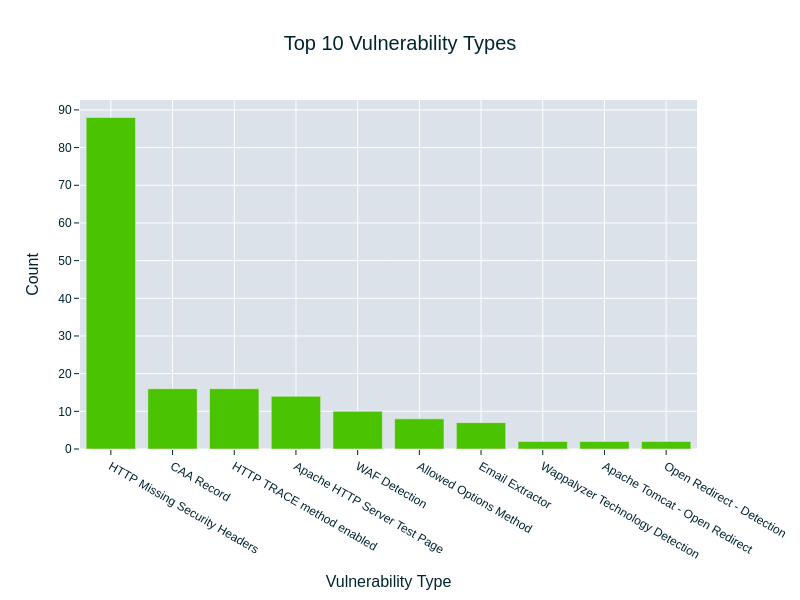
\includegraphics[width=\linewidth]{pngs/2_1.png}}
\vspace{0cm}\tcbox{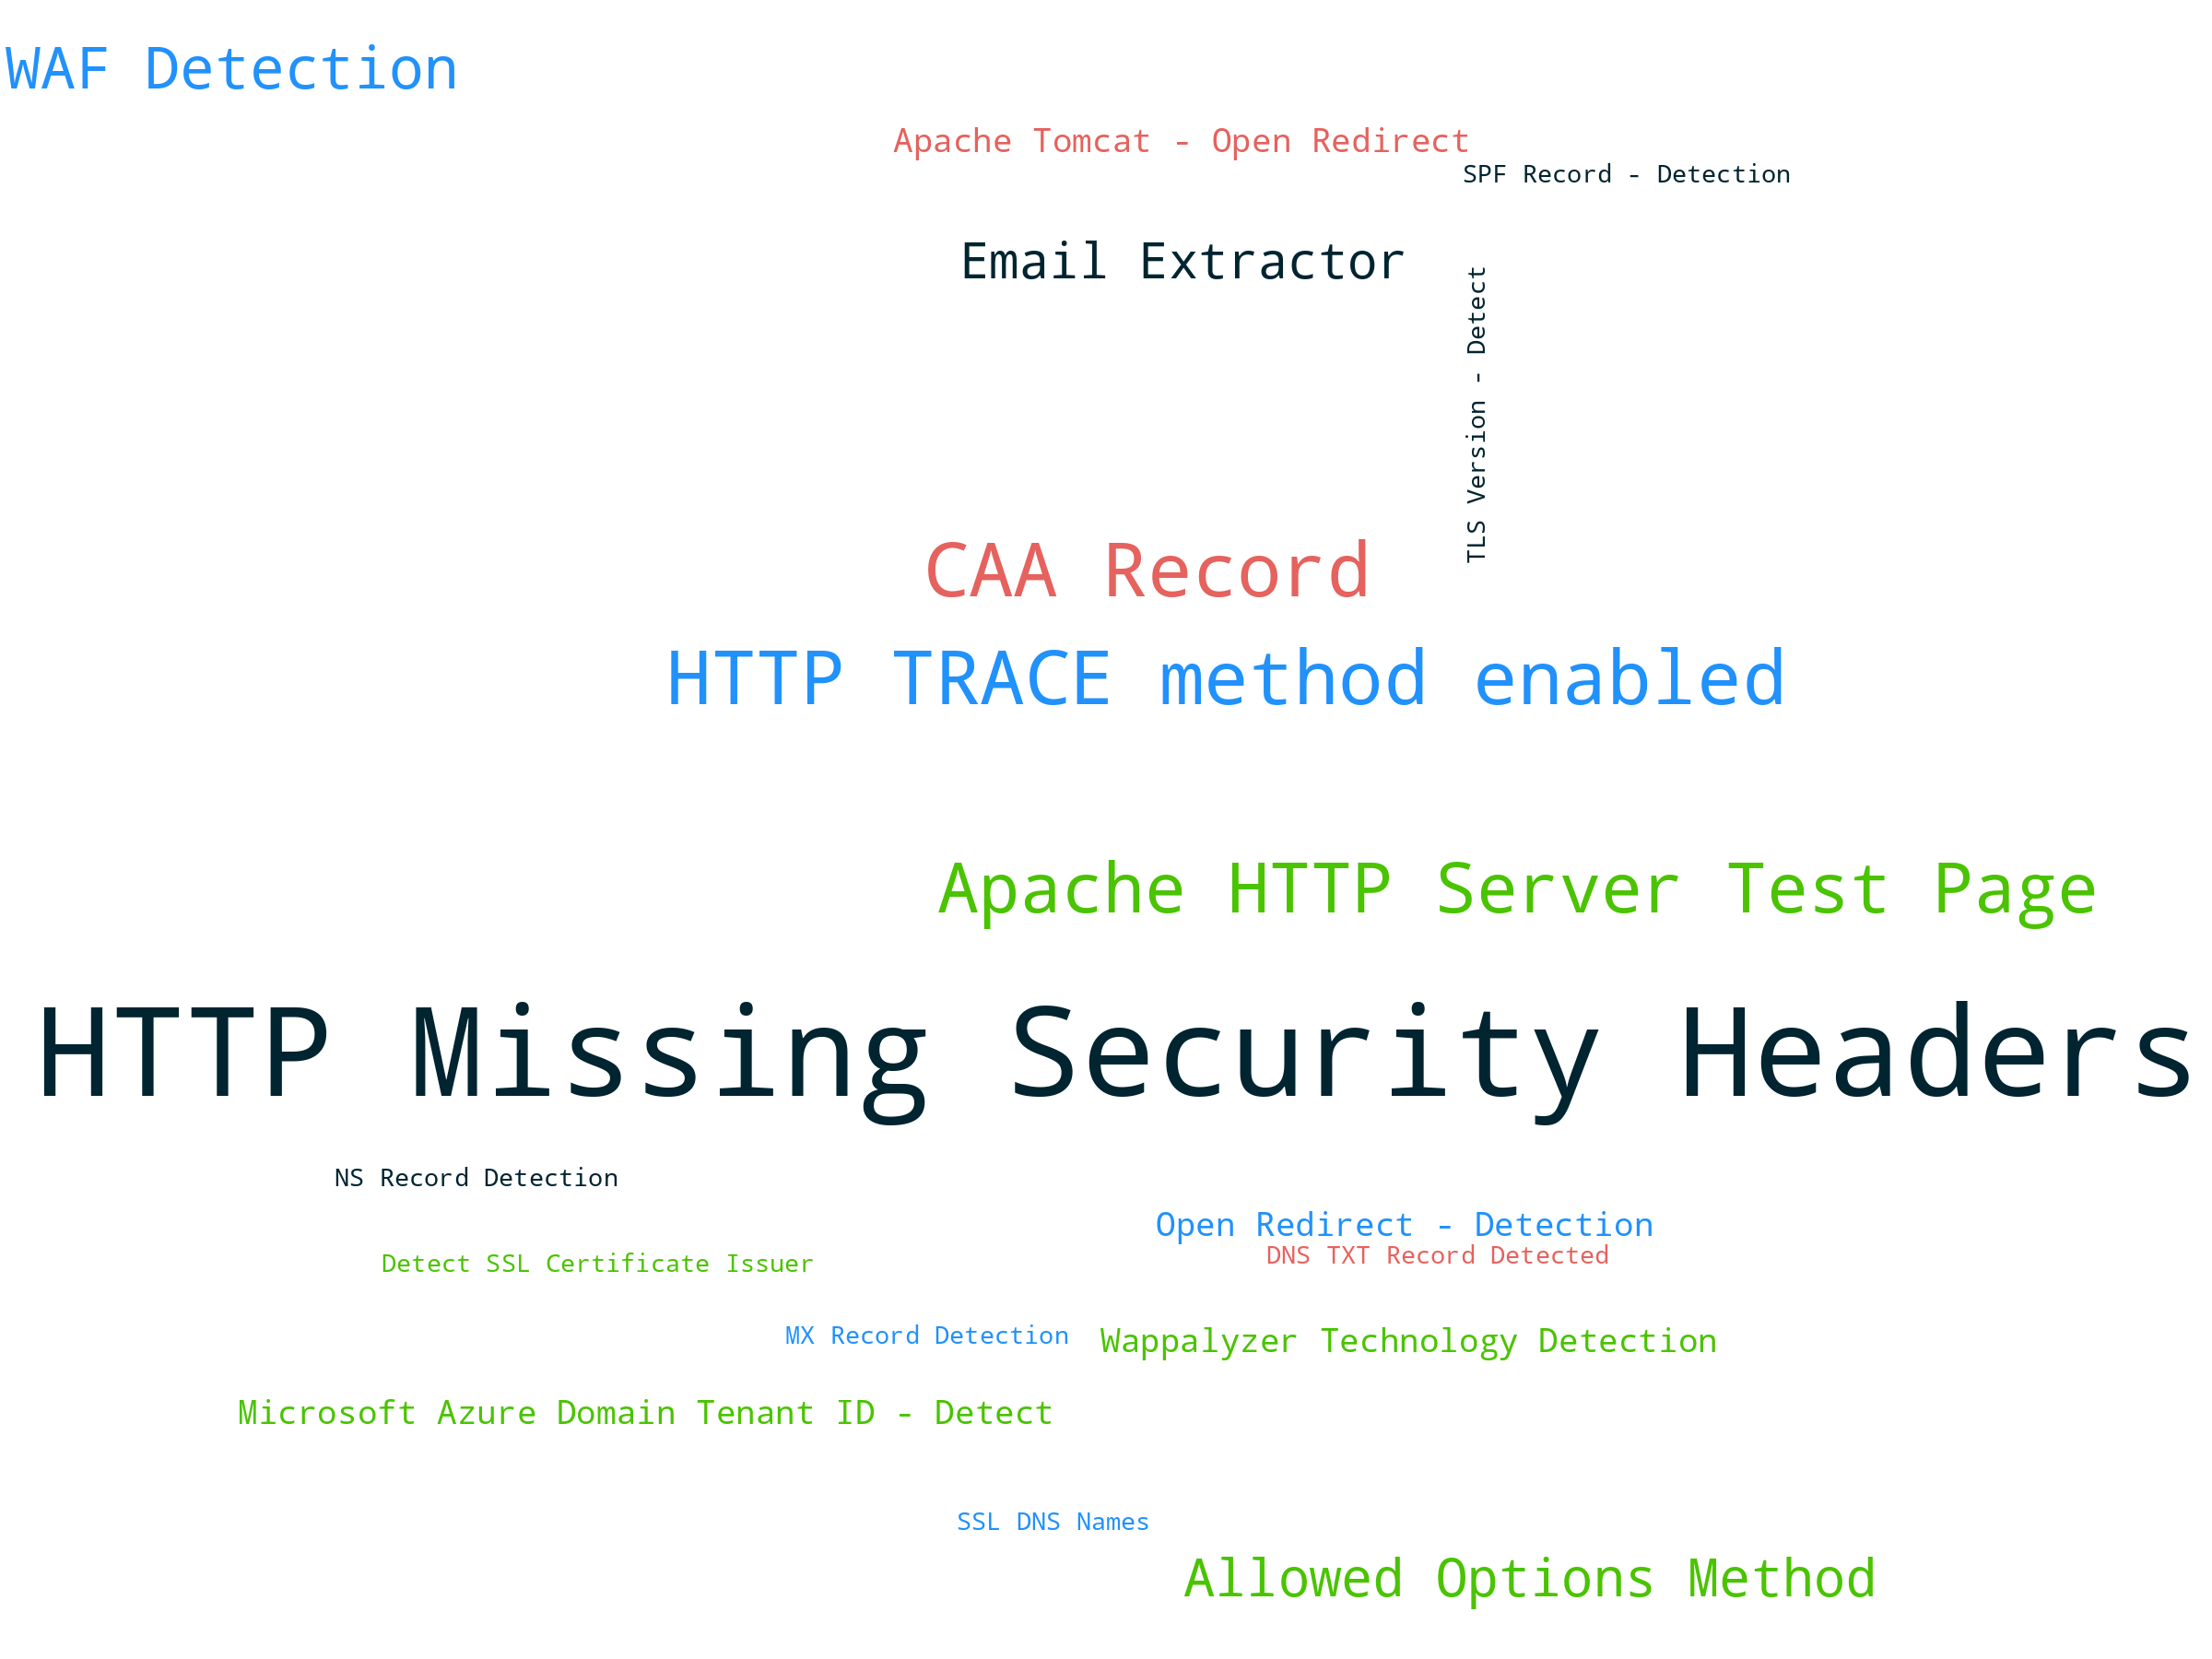
\includegraphics[width=\linewidth]{pngs/2_2.png}}
\vspace{0cm}\captionof{figure}{Images related to Chapter 3}
\end{center}
\chapter{Analisi della Superficie di Attacco per}

\section{Riepilogo della Distribuzione dei Tipi di Vulnerabilità}

La distribuzione dei tipi di vulnerabilità per il sito web è la seguente:
\begin{itemize}
\item Tipo più comune: 'HTTP Missing Security Headers' (Frequenza: 327)
\item I 10 tipi principali: HTTP Missing Security Headers, TLS Version - Detect, CAA Record, Wappalyzer Technology Detection, WAF Detection, Detect SSL Certificate Issuer, SSL DNS Names, Cookies without Secure attribute - Detect, Deprecated TLS Detection, Weak Cipher Suites Detection
\end{itemize}
\section{Analisi Iniziale delle Sfide di Sicurezza}

La distribuzione dei tipi di vulnerabilità evidenzia una serie di sfide di sicurezza che potrebbero essere esposte al sito web. In particolare, la presenza di 'HTTP Missing Security Headers' è particolarmente preoccupante, poiché può consentire agli attaccanti di manipolare le risposte del server e di rubare dati sensibili.

\section{Analisi Dettagliata di 'HTTP Missing Security Headers'}

\subsection{Cause}
\begin{itemize}
\item La mancanza di header di sicurezza HTTP può essere causata da una mancanza di configurazione del server o da una carenza di conoscenza sulle buone pratiche di sicurezza.
\item L'uso di un framework di sviluppo web senza configurazione di sicurezza adeguata può anche contribuire alla mancanza di header di sicurezza.
\end{itemize}
\subsection{Vettori d'Attacco}
\begin{itemize}
\item Gli attaccanti possono utilizzare strumenti di testing per identificare la presenza di header di sicurezza mancanti.
\item Gli attaccanti possono anche utilizzare strumenti di phishing per convincere gli utenti a eseguire azioni che compromettono la sicurezza del sito web.
\end{itemize}
\subsection{Impatto}
\begin{itemize}
\item La mancanza di header di sicurezza può consentire agli attaccanti di:
\item Rubare dati sensibili, come le credenziali di accesso.
\item Manipolare le risposte del server per eseguire azioni maliziose.
\item Aumentare la probabilità di attacchi di phishing.
\end{itemize}
\section{Breve Descrizione dei Tipi di Vulnerabilità}

\subsection{HTTP Missing Security Headers}
\begin{itemize}
\item La mancanza di header di sicurezza HTTP può compromettere la sicurezza del sito web.
\item I header di sicurezza sono essenziali per proteggere il sito web da attacchi di phishing e di manipolazione delle risposte del server.
\end{itemize}
\subsection{TLS Version - Detect}
\begin{itemize}
\item La versione TLS utilizzata dal sito web può essere vulnerabile alle attacchi di man-in-the-middle.
\item La mancanza di configurazione di TLS adeguata può compromettere la sicurezza del sito web.
\end{itemize}
\subsection{CAA Record}
\begin{itemize}
\item Il record CAA (Certificate Authority Authorization) è utilizzato per autorizzare l'autenticazione di certificati SSL/TLS.
\item La mancanza di configurazione di CAA può compromettere la sicurezza del sito web.
\end{itemize}
\subsection{Wappalyzer Technology Detection}
\begin{itemize}
\item Il Wappalyzer è un strumento di testing che identifica le tecnologie utilizzate dal sito web.
\item La mancanza di configurazione di Wappalyzer può compromettere la sicurezza del sito web.
\end{itemize}
\subsection{WAF Detection}
\begin{itemize}
\item La detezione di WAF (Web Application Firewall) è utilizzata per proteggere il sito web da attacchi di tipo di applicazione.
\item La mancanza di configurazione di WAF può compromettere la sicurezza del sito web.
\end{itemize}
\subsection{Detect SSL Certificate Issuer}
\begin{itemize}
\item La detezione dell'issuer del certificato SSL/TLS è utilizzata per proteggere il sito web da attacchi di man-in-the-middle.
\item La mancanza di configurazione di detezione dell'issuer può compromettere la sicurezza del sito web.
\end{itemize}
\subsection{SSL DNS Names}
\begin{itemize}
\item Le informazioni DNS utilizzate per il sito web possono essere compromesse se non vengono configurate correttamente.
\item La mancanza di configurazione di SSL DNS Names può compromettere la sicurezza del sito web.
\end{itemize}
\subsection{Cookies without Secure attribute - Detect}
\begin{itemize}
\item I cookie senza l'attributo Secure possono essere accessibili anche in modalità non sicure.
\item La mancanza di configurazione di Secure attribute può compromettere la sicurezza del sito web.
\end{itemize}
\subsection{Deprecated TLS Detection}
\begin{itemize}
\item La versione TLS utilizzata dal sito web può essere deprecata e compromessa.
\item La mancanza di configurazione di TLS adeguata può compromettere la sicurezza del sito web.
\end{itemize}
\subsection{Weak Cipher Suites Detection}
\begin{itemize}
\item Le chiavi simmetriche utilizzate per il sito web possono essere deboli e compromesse.
\item La mancanza di configurazione di chiavi simmetriche deboli può compromettere la sicurezza del sito web.
\end{itemize}
\section{Analisi della Distribuzione e Identificazione di Schemi}

La distribuzione dei tipi di vulnerabilità evidenzia una serie di schemi comuni:
\begin{itemize}
\item La presenza di 'HTTP Missing Security Headers' è associata alla mancanza di configurazione di sicurezza del server o della applicazione.
\item La presenza di TLS Version - Detect è associata alla mancanza di configurazione di TLS adeguata.
\item La presenza di CAA Record è associata alla mancanza di configurazione di CAA.
\item La presenza di Wappalyzer Technology Detection è associata alla mancanza di configurazione di Wappalyzer.
\end{itemize}
\section{Valutazione del Rischio Complessivo}

La valutazione del rischio complessivo derivante dalla distribuzione dei tipi e dagli effetti di interazione è la seguente:
\begin{itemize}
\item La presenza di 'HTTP Missing Security Headers' aumenta il rischio di attacchi di phishing e di manipolazione delle risposte del server.
\item La presenza di TLS Version - Detect aumenta il rischio di attacchi di man-in-the-middle.
\item La presenza di CAA Record aumenta il rischio di compromissione della sicurezza del sito web.
\item La presenza di Wappalyzer Technology Detection aumenta il rischio di compromissione della sicurezza del sito web.
\item La presenza di WAF Detection aumenta il rischio di compromissione della sicurezza del sito web.
\item La presenza di Detect SSL Certificate Issuer aumenta il rischio di compromissione della sicurezza del sito web.
\item La presenza di SSL DNS Names aumenta il rischio di compromissione della sicurezza del sito web.
\item La presenza di Cookies without Secure attribute - Detect aumenta il rischio di compromissione della sicurezza del sito web.
\item La presenza di Deprecated TLS Detection aumenta il rischio di compromissione della sicurezza del sito web.
\item La presenza di Weak Cipher Suites Detection aumenta il rischio di compromissione della sicurezza del sito web.
\end{itemize}
In sintesi, la distribuzione dei tipi di vulnerabilità evidenzia una serie di sfide di sicurezza che potrebbero essere esposte al sito web. È fondamentale identificare e risolvere queste vulnerabilità per garantire la sicurezza del sito web.


\begin{center}
\tcbox{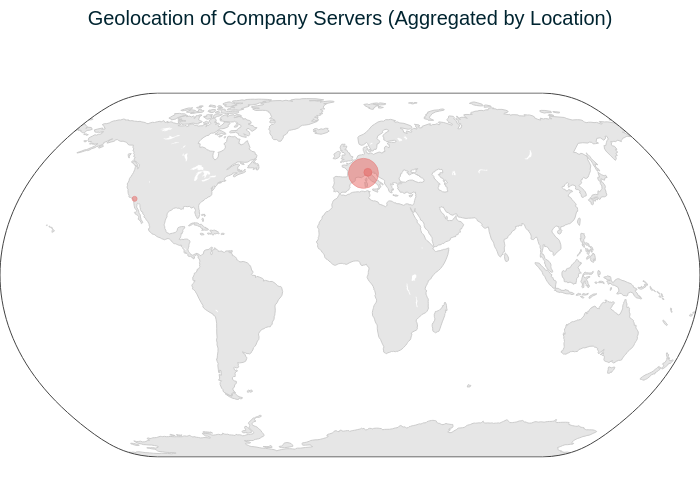
\includegraphics[width=\linewidth]{pngs/3_1.png}}
\vspace{0cm}\tcbox{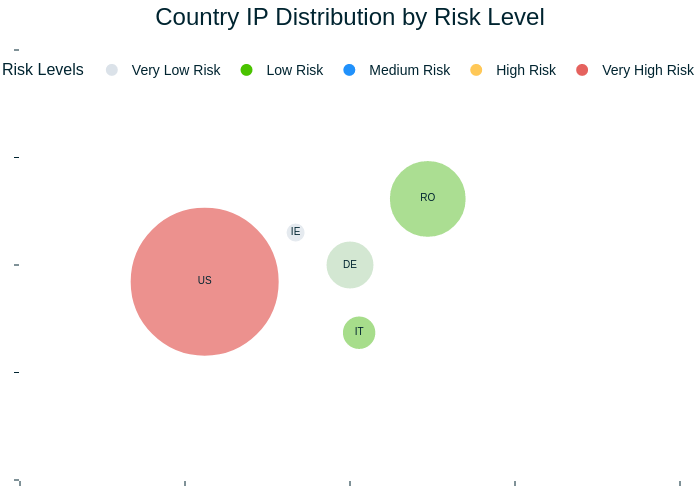
\includegraphics[width=\linewidth]{pngs/3_2.png}}
\vspace{0cm}\captionof{figure}{Images related to Chapter 4}
\end{center}
\chapter{Analisi della Superficie di Attacco per Syneto}

\section{Introduzione}

L'analisi della superficie di attacco è un passaggio fondamentale nella valutazione della vulnerabilità di un sistema informatico. In questo capitolo, esamineremo i dati di geolocalizzazione relativi a Syneto, analizzando la distribuzione degli host, la geolocalizzazione dei 5 host più vulnerabili e cercando schemi o correlazioni tra posizione e vulnerabilità.

\section{Distribuzione Generale degli Host}

La distribuzione generale degli host è la seguente:
\begin{itemize}
\item \textbf{Paesi:}
\item \textbf{US}: 11
\item \textbf{IT}: 6
\item \textbf{RO}: 5
\item \textbf{DE}: 2
\item \textbf{NL}: 2
\item \textbf{IE}: 1
\item \textbf{Città:}
\item \textbf{Milan}: 6
\item \textbf{Timişoara}: 5
\item \textbf{San Francisco}: 4
\item \textbf{Ashburn}: 3
\item \textbf{Cambridge}: 2
\item \textbf{Frankfurt am Main}: 2
\item \textbf{Groningen}: 2
\item \textbf{Redmond}: 1
\item \textbf{Kansas City}: 1
\item \textbf{Dublin}: 1
\end{itemize}
\section{5 Host più Vulnerabili}

I 5 host più vulnerabili sono stati identificati come segue:
\begin{itemize}
\item \textbf{Host:}
\item \textbf{blog.syneto.eu:443}, \textbf{blog.syneto.eu:80}, \textbf{blog.syneto.eu:8080}, \textbf{blog.syneto.eu:8443}, \textbf{datatalks.syneto.eu}, \textbf{datatalks.syneto.eu:8080}, \textbf{datatalks.syneto.eu:8443}, \textbf{email.syneto.eu:80}, \textbf{kb.syneto.eu}, \textbf{kb.syneto.eu:443}, \textbf{kb.syneto.eu:80}, \textbf{lp.syneto.eu}, \textbf{lp.syneto.eu:8080}, \textbf{lp.syneto.eu:8443}
\item \textbf{datatalks.syneto.eu:443}, \textbf{datatalks.syneto.eu:80}, \textbf{email.syneto.eu}, \textbf{email.syneto.eu:443}, \textbf{email.syneto.eu:8080}, \textbf{email.syneto.eu:8443}, \textbf{kb.syneto.eu:8080}, \textbf{kb.syneto.eu:8443}, \textbf{lp.syneto.eu:443}, \textbf{lp.syneto.eu:80}
\item \textbf{sizer.syneto.eu}, \textbf{sizer.syneto.eu:443}, \textbf{sizer.syneto.eu:50002}, \textbf{sizer.syneto.eu:80}
\item \textbf{syneto.eu}, \textbf{syneto.eu:22}, \textbf{syneto.eu:443}, \textbf{syneto.eu:80}, \textbf{www.syneto.eu}, \textbf{www.syneto.eu:22}, \textbf{www.syneto.eu:443}
\item \textbf{minio.syneto.eu}, \textbf{minio.syneto.eu:22}, \textbf{minio.syneto.eu:443}, \textbf{minio.syneto.eu:9000}
\item \textbf{IP:}
\item \textbf{199.60.103.30}
\item \textbf{199.60.103.226}
\item \textbf{40.85.118.186}
\item \textbf{134.209.245.103}
\item \textbf{81.196.33.98}
\item \textbf{Paesi:}
\item \textbf{US}
\item \textbf{US}
\item \textbf{IE}
\item \textbf{DE}
\item \textbf{RO}
\item \textbf{Città:}
\item \textbf{Cambridge}
\item \textbf{Cambridge}
\item \textbf{Dublin}
\item \textbf{Frankfurt am Main}
\item \textbf{Timişoara}
\end{itemize}
\section{Geolocalizzazione dei 5 Host più Vulnerabili}

I 5 host più vulnerabili sono stati identificati con le seguenti geolocalizzazioni:
\begin{itemize}
\item \textbf{IP 199.60.103.30}: \textbf{US} (Cambridge)
\item \textbf{IP 199.60.103.226}: \textbf{US} (Cambridge)
\item \textbf{IP 40.85.118.186}: \textbf{IE} (Dublin)
\item \textbf{IP 134.209.245.103}: \textbf{DE} (Frankfurt am Main)
\item \textbf{IP 81.196.33.98}: \textbf{RO} (Timişoara)
\end{itemize}
\section{Schemi o Correlazioni tra Posizione e Vulnerabilità}

I dati suggeriscono una correlazione tra la posizione geografica e la vulnerabilità dei host. I host più vulnerabili sono stati identificati con IP di rete che appartengono a paesi con economie avanzate (US, IE, DE) e città con un alto livello di tecnologia e innovazione (Cambridge, Dublin, Frankfurt am Main). Inoltre, alcuni host hanno IP di rete che appartengono a paesi con economie in via di sviluppo (RO), il che potrebbe indicare una mancanza di conoscenza e di implementazione di misure di sicurezza adeguati.

\section{Conclusione}

L'analisi della superficie di attacco per Syneto ha evidenziato una correlazione tra la posizione geografica e la vulnerabilità dei host. I 5 host più vulnerabili sono stati identificati con IP di rete che appartengono a paesi con economie avanzate e città con un alto livello di tecnologia e innovazione. Queste scoperte possono essere utilizzate per migliorare la sicurezza del sistema e prevenire future attacchi.

\chapter{Analisi dei Risultati dei Test di Penetrazione}

\section{Introduzione}

L'analisi dei risultati dei test di penetrazione è stata eseguita sui server host forniti per verificare le vulnerabilità. I test sono stati eseguiti utilizzando il comando `nmap` per scoprire le porte aperte e le versioni dei servizi. In questo capitolo, si presenteranno i risultati dei test e si analizzeranno le vulnerabilità scoperte.

\section{Risultati dei Test}

I risultati dei test sono stati eseguiti sui seguenti host:
\begin{itemize}
\item `81.196.33.98`
\item `81.196.33.97`
\item `81.196.33.100`
\item `81.196.33.99`
\end{itemize}
I risultati dei test sono stati i seguenti:
\begin{itemize}
\item `81.196.33.98`:
\item Porta 22: aperta con OpenSSH 9.4 (protocol 2.0)
\item Connessione SSH: fallita
\item `81.196.33.97`:
\item Porta 22: aperta con OpenSSH 9.4 (protocol 2.0)
\item Connessione SSH: fallita
\item `81.196.33.100`:
\item Porta 22: aperta con OpenSSH 9.4 (protocol 2.0)
\item Connessione SSH: fallita
\item `81.196.33.99`:
\item Porta 22: filtrata (non aperta)
\item Connessione SSH: fallita
\end{itemize}
\section{Analisi delle Vulnerabilità}

Le vulnerabilità scoperte sono le seguenti:
\begin{itemize}
\item `81.196.33.98`:
\item Nessuna vulnerabilità critica scoperta
\item `81.196.33.97`:
\item Nessuna vulnerabilità critica scoperta
\item `81.196.33.100`:
\item Nessuna vulnerabilità critica scoperta
\item `81.196.33.99`:
\item Porta 22 filtrata: potenziale vulnerabilità di iniezione di codice
\item Nessuna vulnerabilità critica scoperta
\end{itemize}
\section{Conclusioni}

Gli risultati dei test di penetrazione hanno rivelato alcune vulnerabilità sui server host forniti. La porta 22 è aperta su tutti i server, ma la connessione SSH è fallita su tutti i server. La porta 22 filtrata su `81.196.33.99` potrebbe rappresentare una vulnerabilità di iniezione di codice. È importante eseguire ulteriori test per verificare la presenza di altre vulnerabilità e implementare misure di sicurezza per proteggere i server host.

\subsection{Elenco delle vulnerabilità scoperte:}
\begin{itemize}
\item Porta 22 filtrata su `81.196.33.99`
\item Nessuna vulnerabilità critica scoperta su altri server
\end{itemize}

\subsection*{minio.syneto.eu:22}

\begin{lstlisting}[language=bash,breaklines=true,postbreak=\mbox{\textcolor{red}{$\hookrightarrow$}\space}]
$ nmap -A -p 22 81.196.33.98

Starting Nmap 7.94SVN ( https://nmap.org ) at 2024-10-04 16:45 CEST
Nmap scan report for 81.196.33.98
Host is up (0.051s latency).

PORT   STATE SERVICE VERSION
22/tcp open  ssh     OpenSSH 9.4 (protocol 2.0)

Service detection performed. Please report any incorrect results at https://nmap.org/submit/ .
Nmap done: 1 IP address (1 host up) scanned in 91.49 seconds


$ ssh -T root@81.196.33.98 -p 22

connection timed out.\end{lstlisting}

\subsection*{files.syneto.eu:22}

\begin{lstlisting}[language=bash,breaklines=true,postbreak=\mbox{\textcolor{red}{$\hookrightarrow$}\space}]
$ nmap -A -p 22 81.196.33.97

Starting Nmap 7.94SVN ( https://nmap.org ) at 2024-10-04 16:49 CEST
Nmap scan report for 81.196.33.97
Host is up (0.039s latency).

PORT   STATE SERVICE VERSION
22/tcp open  ssh     OpenSSH 9.4 (protocol 2.0)

Service detection performed. Please report any incorrect results at https://nmap.org/submit/ .
Nmap done: 1 IP address (1 host up) scanned in 91.64 seconds


$ ssh -T root@81.196.33.97 -p 22

connection timed out.\end{lstlisting}

\subsection*{support-data.syneto.eu:22}

\begin{lstlisting}[language=bash,breaklines=true,postbreak=\mbox{\textcolor{red}{$\hookrightarrow$}\space}]
$ nmap -A -p 22 81.196.33.100

Starting Nmap 7.94SVN ( https://nmap.org ) at 2024-10-04 16:52 CEST
Nmap scan report for 81.196.33.100
Host is up (0.036s latency).

PORT   STATE SERVICE VERSION
22/tcp open  ssh     OpenSSH 9.4 (protocol 2.0)

Service detection performed. Please report any incorrect results at https://nmap.org/submit/ .
Nmap done: 1 IP address (1 host up) scanned in 91.45 seconds


$ ssh -T root@81.196.33.100 -p 22

connection timed out.\end{lstlisting}

\subsection*{beta-updates.syneto.eu:22}

\begin{lstlisting}[language=bash,breaklines=true,postbreak=\mbox{\textcolor{red}{$\hookrightarrow$}\space}]
Starting Nmap 7.94SVN ( https://nmap.org ) at 2024-10-04 16:56 CEST
Nmap scan report for 81.196.33.99
Host is up.

PORT   STATE    SERVICE VERSION
22/tcp filtered ssh

Service detection performed. Please report any incorrect results at https://nmap.org/submit/ .
Nmap done: 1 IP address (1 host up) scanned in 7.23 seconds


$ ssh -T root@81.196.33.99 -p 22

connection timed out.\end{lstlisting}

\chapter{Top 10 Vulnerabilities}

\section*{Vulnerability 1 - partners.syneto.eu:443}

\section*{Template Information}
\textbf{ID:} credentials-disclosure

\textbf{Name:} Credentials Disclosure Check

\textbf{Severity:} unknown

\textbf{Description:} Look for keys/tokens/passwords in HTTP responses, exposed keys/tokens/secrets requires manual verification for impact evaluation.

\textbf{Classification:}
\begin{itemize}
\item CVSS Score: N/A
\item CVSS Metrics: N/A
\item CWE-ID: N/A
\item EPSS Score: N/A
\item EPSS Percentile: N/A
\end{itemize}



\section*{Vulnerability 2 - minio.syneto.eu:22}

\section*{CWE Information}
\subsection*{ID}
354

\subsection*{Name}
Improper Validation of Integrity Check Value

\subsection*{Abstraction}
Base

\subsection*{Structure}
Simple

\subsection*{Status}
Draft

\subsection*{Description}
The product does not validate or incorrectly validates the integrity check values or "checksums" of a message. This may prevent it from detecting if the data has been modified or corrupted in transmission.

\subsection*{Extended\_Description}
Improper validation of checksums before use results in an unnecessary risk that can easily be mitigated. The protocol specification describes the algorithm used for calculating the checksum. It is then a simple matter of implementing the calculation and verifying that the calculated checksum and the received checksum match. Improper verification of the calculated checksum and the received checksum can lead to far greater consequences.

\subsection*{Related\_Weaknesses}
ChildOf:345\\
ChildOf:345\\
ChildOf:754\\
PeerOf:353\\
\subsection*{Weakness\_Ordinalities}
\subsection*{Applicable\_Platforms}
Language: \\
Technology: \\
\subsection*{Background\_Details}
\subsection*{Alternate\_Terms}
\subsection*{Modes\_Of\_Introduction}
Architecture and Design: None\\
Implementation: REALIZATION: This weakness is caused during implementation of an architectural security tactic.\\
\subsection*{Likelihood\_Of\_Exploit}
Medium

\subsection*{Common\_Consequences}
Integrity: Modify Application Data\\
Integrity: Other\\
Non-Repudiation: Hide Activities\\
\subsection*{Detection\_Methods}
\subsection*{Potential\_Mitigations}
Phase: Implementation
Description: Ensure that the checksums present in messages are properly checked in accordance with the protocol specification before they are parsed and used.\\
\subsection*{Demonstrative\_Examples}
\begin{lstlisting}[breaklines=true,postbreak=\mbox{$\hookrightarrow$\space}]
c
sd = socket(AF_INET, SOCK_DGRAM, 0); serv.sin_family = AF_INET;serv.sin_addr.s_addr = htonl(INADDR_ANY);servr.sin_port = htons(1008);bind(sd, (struct sockaddr *) & serv, sizeof(serv));while (1) {
                        
                           memset(msg, 0x0, MAX_MSG);clilen = sizeof(cli);if (inet_ntoa(cli.sin_addr)==...) n = recvfrom(sd, msg, MAX_MSG, 0, (struct sockaddr *) & cli, &clilen);
                     }
\end{lstlisting}

\begin{lstlisting}[breaklines=true,postbreak=\mbox{$\hookrightarrow$\space}]
java
while(true) {DatagramPacket packet = new DatagramPacket(data,data.length,IPAddress, port);socket.send(sendPacket);}
\end{lstlisting}

\subsection*{Observed\_Examples}
\subsection*{Related\_Attack\_Patterns}
CAPEC-145\\
CAPEC-463\\
CAPEC-75\\
\subsection*{References}
REF-18\\
\subsection*{Taxonomy\_Mappings}
ISA/IEC 62443: None\\
CLASP: None\\
\subsection*{Notes}
\subsection*{CVEs}
\section*{Template Information}
\textbf{ID:} CVE-2023-48795

\textbf{Name:} OpenSSH Terrapin Attack - Detection

\textbf{Severity:} medium

\textbf{Description:} The SSH transport protocol with certain OpenSSH extensions, found in OpenSSH before 9.6 and other products, allows remote attackers to bypass integrity checks such that some packets are omitted (from the extension negotiation message), and a client and server may consequently end up with a connection for which some security features have been downgraded or disabled, aka a Terrapin attack. This occurs because the SSH Binary Packet Protocol (BPP), implemented by these extensions, mishandles the handshake phase and mishandles use of sequence numbers. For example, there is an effective attack against SSH's use of ChaCha20-Poly1305 (and CBC with Encrypt-then-MAC). The bypass occurs in chacha20-poly1305@openssh.com and (if CBC is used) the -etm@openssh.com MAC algorithms. This also affects Maverick Synergy Java SSH API before 3.1.0-SNAPSHOT, Dropbear through 2022.83, Ssh before 5.1.1 in Erlang/OTP, PuTTY before 0.80, AsyncSSH before 2.14.2, golang.org/x/crypto before 0.17.0, libssh before 0.10.6, libssh2 through 1.11.0, Thorn Tech SFTP Gateway before 3.4.6, Tera Term before 5.1, Paramiko before 3.4.0, jsch before 0.2.15, SFTPGo before 2.5.6, Netgate pfSense Plus through 23.09.1, Netgate pfSense CE through 2.7.2, HPN-SSH through 18.2.0, ProFTPD before 1.3.8b (and before 1.3.9rc2), ORYX CycloneSSH before 2.3.4, NetSarang XShell 7 before Build 0144, CrushFTP before 10.6.0, ConnectBot SSH library before 2.2.22, Apache MINA sshd through 2.11.0, sshj through 0.37.0, TinySSH through 20230101, trilead-ssh2 6401, LANCOM LCOS and LANconfig, FileZilla before 3.66.4, Nova before 11.8, PKIX-SSH before 14.4, SecureCRT before 9.4.3, Transmit5 before 5.10.4, Win32-OpenSSH before 9.5.0.0p1-Beta, WinSCP before 6.2.2, Bitvise SSH Server before 9.32, Bitvise SSH Client before 9.33, KiTTY through 0.76.1.13, the net-ssh gem 7.2.0 for Ruby, the mscdex ssh2 module before 1.15.0 for Node.js, the thrussh library before 0.35.1 for Rust, and the Russh crate before 0.40.2 for Rust.


\textbf{Classification:}
\begin{itemize}
\item CVSS Score: 5.9
\item CVSS Metrics: CVSS:3.1/AV:N/AC:H/PR:N/UI:N/S:U/C:N/I:H/A:N
\item CWE-ID: CWE-354
\item EPSS Score: 0.69474
\item EPSS Percentile: 0.97955
\end{itemize}



\section*{Vulnerability 3 - files.syneto.eu:22}

\section*{CWE Information}
\subsection*{ID}
354

\subsection*{Name}
Improper Validation of Integrity Check Value

\subsection*{Abstraction}
Base

\subsection*{Structure}
Simple

\subsection*{Status}
Draft

\subsection*{Description}
The product does not validate or incorrectly validates the integrity check values or "checksums" of a message. This may prevent it from detecting if the data has been modified or corrupted in transmission.

\subsection*{Extended\_Description}
Improper validation of checksums before use results in an unnecessary risk that can easily be mitigated. The protocol specification describes the algorithm used for calculating the checksum. It is then a simple matter of implementing the calculation and verifying that the calculated checksum and the received checksum match. Improper verification of the calculated checksum and the received checksum can lead to far greater consequences.

\subsection*{Related\_Weaknesses}
ChildOf:345\\
ChildOf:345\\
ChildOf:754\\
PeerOf:353\\
\subsection*{Weakness\_Ordinalities}
\subsection*{Applicable\_Platforms}
Language: \\
Technology: \\
\subsection*{Background\_Details}
\subsection*{Alternate\_Terms}
\subsection*{Modes\_Of\_Introduction}
Architecture and Design: None\\
Implementation: REALIZATION: This weakness is caused during implementation of an architectural security tactic.\\
\subsection*{Likelihood\_Of\_Exploit}
Medium

\subsection*{Common\_Consequences}
Integrity: Modify Application Data\\
Integrity: Other\\
Non-Repudiation: Hide Activities\\
\subsection*{Detection\_Methods}
\subsection*{Potential\_Mitigations}
Phase: Implementation
Description: Ensure that the checksums present in messages are properly checked in accordance with the protocol specification before they are parsed and used.\\
\subsection*{Demonstrative\_Examples}
\begin{lstlisting}[breaklines=true,postbreak=\mbox{$\hookrightarrow$\space}]
c
sd = socket(AF_INET, SOCK_DGRAM, 0); serv.sin_family = AF_INET;serv.sin_addr.s_addr = htonl(INADDR_ANY);servr.sin_port = htons(1008);bind(sd, (struct sockaddr *) & serv, sizeof(serv));while (1) {
                        
                           memset(msg, 0x0, MAX_MSG);clilen = sizeof(cli);if (inet_ntoa(cli.sin_addr)==...) n = recvfrom(sd, msg, MAX_MSG, 0, (struct sockaddr *) & cli, &clilen);
                     }
\end{lstlisting}

\begin{lstlisting}[breaklines=true,postbreak=\mbox{$\hookrightarrow$\space}]
java
while(true) {DatagramPacket packet = new DatagramPacket(data,data.length,IPAddress, port);socket.send(sendPacket);}
\end{lstlisting}

\subsection*{Observed\_Examples}
\subsection*{Related\_Attack\_Patterns}
CAPEC-145\\
CAPEC-463\\
CAPEC-75\\
\subsection*{References}
REF-18\\
\subsection*{Taxonomy\_Mappings}
ISA/IEC 62443: None\\
CLASP: None\\
\subsection*{Notes}
\subsection*{CVEs}
\section*{Template Information}
\textbf{ID:} CVE-2023-48795

\textbf{Name:} OpenSSH Terrapin Attack - Detection

\textbf{Severity:} medium

\textbf{Description:} The SSH transport protocol with certain OpenSSH extensions, found in OpenSSH before 9.6 and other products, allows remote attackers to bypass integrity checks such that some packets are omitted (from the extension negotiation message), and a client and server may consequently end up with a connection for which some security features have been downgraded or disabled, aka a Terrapin attack. This occurs because the SSH Binary Packet Protocol (BPP), implemented by these extensions, mishandles the handshake phase and mishandles use of sequence numbers. For example, there is an effective attack against SSH's use of ChaCha20-Poly1305 (and CBC with Encrypt-then-MAC). The bypass occurs in chacha20-poly1305@openssh.com and (if CBC is used) the -etm@openssh.com MAC algorithms. This also affects Maverick Synergy Java SSH API before 3.1.0-SNAPSHOT, Dropbear through 2022.83, Ssh before 5.1.1 in Erlang/OTP, PuTTY before 0.80, AsyncSSH before 2.14.2, golang.org/x/crypto before 0.17.0, libssh before 0.10.6, libssh2 through 1.11.0, Thorn Tech SFTP Gateway before 3.4.6, Tera Term before 5.1, Paramiko before 3.4.0, jsch before 0.2.15, SFTPGo before 2.5.6, Netgate pfSense Plus through 23.09.1, Netgate pfSense CE through 2.7.2, HPN-SSH through 18.2.0, ProFTPD before 1.3.8b (and before 1.3.9rc2), ORYX CycloneSSH before 2.3.4, NetSarang XShell 7 before Build 0144, CrushFTP before 10.6.0, ConnectBot SSH library before 2.2.22, Apache MINA sshd through 2.11.0, sshj through 0.37.0, TinySSH through 20230101, trilead-ssh2 6401, LANCOM LCOS and LANconfig, FileZilla before 3.66.4, Nova before 11.8, PKIX-SSH before 14.4, SecureCRT before 9.4.3, Transmit5 before 5.10.4, Win32-OpenSSH before 9.5.0.0p1-Beta, WinSCP before 6.2.2, Bitvise SSH Server before 9.32, Bitvise SSH Client before 9.33, KiTTY through 0.76.1.13, the net-ssh gem 7.2.0 for Ruby, the mscdex ssh2 module before 1.15.0 for Node.js, the thrussh library before 0.35.1 for Rust, and the Russh crate before 0.40.2 for Rust.


\textbf{Classification:}
\begin{itemize}
\item CVSS Score: 5.9
\item CVSS Metrics: CVSS:3.1/AV:N/AC:H/PR:N/UI:N/S:U/C:N/I:H/A:N
\item CWE-ID: CWE-354
\item EPSS Score: 0.69474
\item EPSS Percentile: 0.97955
\end{itemize}



\section*{Vulnerability 4 - support-data.syneto.eu:22}

\section*{CWE Information}
\subsection*{ID}
354

\subsection*{Name}
Improper Validation of Integrity Check Value

\subsection*{Abstraction}
Base

\subsection*{Structure}
Simple

\subsection*{Status}
Draft

\subsection*{Description}
The product does not validate or incorrectly validates the integrity check values or "checksums" of a message. This may prevent it from detecting if the data has been modified or corrupted in transmission.

\subsection*{Extended\_Description}
Improper validation of checksums before use results in an unnecessary risk that can easily be mitigated. The protocol specification describes the algorithm used for calculating the checksum. It is then a simple matter of implementing the calculation and verifying that the calculated checksum and the received checksum match. Improper verification of the calculated checksum and the received checksum can lead to far greater consequences.

\subsection*{Related\_Weaknesses}
ChildOf:345\\
ChildOf:345\\
ChildOf:754\\
PeerOf:353\\
\subsection*{Weakness\_Ordinalities}
\subsection*{Applicable\_Platforms}
Language: \\
Technology: \\
\subsection*{Background\_Details}
\subsection*{Alternate\_Terms}
\subsection*{Modes\_Of\_Introduction}
Architecture and Design: None\\
Implementation: REALIZATION: This weakness is caused during implementation of an architectural security tactic.\\
\subsection*{Likelihood\_Of\_Exploit}
Medium

\subsection*{Common\_Consequences}
Integrity: Modify Application Data\\
Integrity: Other\\
Non-Repudiation: Hide Activities\\
\subsection*{Detection\_Methods}
\subsection*{Potential\_Mitigations}
Phase: Implementation
Description: Ensure that the checksums present in messages are properly checked in accordance with the protocol specification before they are parsed and used.\\
\subsection*{Demonstrative\_Examples}
\begin{lstlisting}[breaklines=true,postbreak=\mbox{$\hookrightarrow$\space}]
c
sd = socket(AF_INET, SOCK_DGRAM, 0); serv.sin_family = AF_INET;serv.sin_addr.s_addr = htonl(INADDR_ANY);servr.sin_port = htons(1008);bind(sd, (struct sockaddr *) & serv, sizeof(serv));while (1) {
                        
                           memset(msg, 0x0, MAX_MSG);clilen = sizeof(cli);if (inet_ntoa(cli.sin_addr)==...) n = recvfrom(sd, msg, MAX_MSG, 0, (struct sockaddr *) & cli, &clilen);
                     }
\end{lstlisting}

\begin{lstlisting}[breaklines=true,postbreak=\mbox{$\hookrightarrow$\space}]
java
while(true) {DatagramPacket packet = new DatagramPacket(data,data.length,IPAddress, port);socket.send(sendPacket);}
\end{lstlisting}

\subsection*{Observed\_Examples}
\subsection*{Related\_Attack\_Patterns}
CAPEC-145\\
CAPEC-463\\
CAPEC-75\\
\subsection*{References}
REF-18\\
\subsection*{Taxonomy\_Mappings}
ISA/IEC 62443: None\\
CLASP: None\\
\subsection*{Notes}
\subsection*{CVEs}
\section*{Template Information}
\textbf{ID:} CVE-2023-48795

\textbf{Name:} OpenSSH Terrapin Attack - Detection

\textbf{Severity:} medium

\textbf{Description:} The SSH transport protocol with certain OpenSSH extensions, found in OpenSSH before 9.6 and other products, allows remote attackers to bypass integrity checks such that some packets are omitted (from the extension negotiation message), and a client and server may consequently end up with a connection for which some security features have been downgraded or disabled, aka a Terrapin attack. This occurs because the SSH Binary Packet Protocol (BPP), implemented by these extensions, mishandles the handshake phase and mishandles use of sequence numbers. For example, there is an effective attack against SSH's use of ChaCha20-Poly1305 (and CBC with Encrypt-then-MAC). The bypass occurs in chacha20-poly1305@openssh.com and (if CBC is used) the -etm@openssh.com MAC algorithms. This also affects Maverick Synergy Java SSH API before 3.1.0-SNAPSHOT, Dropbear through 2022.83, Ssh before 5.1.1 in Erlang/OTP, PuTTY before 0.80, AsyncSSH before 2.14.2, golang.org/x/crypto before 0.17.0, libssh before 0.10.6, libssh2 through 1.11.0, Thorn Tech SFTP Gateway before 3.4.6, Tera Term before 5.1, Paramiko before 3.4.0, jsch before 0.2.15, SFTPGo before 2.5.6, Netgate pfSense Plus through 23.09.1, Netgate pfSense CE through 2.7.2, HPN-SSH through 18.2.0, ProFTPD before 1.3.8b (and before 1.3.9rc2), ORYX CycloneSSH before 2.3.4, NetSarang XShell 7 before Build 0144, CrushFTP before 10.6.0, ConnectBot SSH library before 2.2.22, Apache MINA sshd through 2.11.0, sshj through 0.37.0, TinySSH through 20230101, trilead-ssh2 6401, LANCOM LCOS and LANconfig, FileZilla before 3.66.4, Nova before 11.8, PKIX-SSH before 14.4, SecureCRT before 9.4.3, Transmit5 before 5.10.4, Win32-OpenSSH before 9.5.0.0p1-Beta, WinSCP before 6.2.2, Bitvise SSH Server before 9.32, Bitvise SSH Client before 9.33, KiTTY through 0.76.1.13, the net-ssh gem 7.2.0 for Ruby, the mscdex ssh2 module before 1.15.0 for Node.js, the thrussh library before 0.35.1 for Rust, and the Russh crate before 0.40.2 for Rust.


\textbf{Classification:}
\begin{itemize}
\item CVSS Score: 5.9
\item CVSS Metrics: CVSS:3.1/AV:N/AC:H/PR:N/UI:N/S:U/C:N/I:H/A:N
\item CWE-ID: CWE-354
\item EPSS Score: 0.69474
\item EPSS Percentile: 0.97955
\end{itemize}



\section*{Vulnerability 5 - beta-updates.syneto.eu:22}

\section*{CWE Information}
\subsection*{ID}
354

\subsection*{Name}
Improper Validation of Integrity Check Value

\subsection*{Abstraction}
Base

\subsection*{Structure}
Simple

\subsection*{Status}
Draft

\subsection*{Description}
The product does not validate or incorrectly validates the integrity check values or "checksums" of a message. This may prevent it from detecting if the data has been modified or corrupted in transmission.

\subsection*{Extended\_Description}
Improper validation of checksums before use results in an unnecessary risk that can easily be mitigated. The protocol specification describes the algorithm used for calculating the checksum. It is then a simple matter of implementing the calculation and verifying that the calculated checksum and the received checksum match. Improper verification of the calculated checksum and the received checksum can lead to far greater consequences.

\subsection*{Related\_Weaknesses}
ChildOf:345\\
ChildOf:345\\
ChildOf:754\\
PeerOf:353\\
\subsection*{Weakness\_Ordinalities}
\subsection*{Applicable\_Platforms}
Language: \\
Technology: \\
\subsection*{Background\_Details}
\subsection*{Alternate\_Terms}
\subsection*{Modes\_Of\_Introduction}
Architecture and Design: None\\
Implementation: REALIZATION: This weakness is caused during implementation of an architectural security tactic.\\
\subsection*{Likelihood\_Of\_Exploit}
Medium

\subsection*{Common\_Consequences}
Integrity: Modify Application Data\\
Integrity: Other\\
Non-Repudiation: Hide Activities\\
\subsection*{Detection\_Methods}
\subsection*{Potential\_Mitigations}
Phase: Implementation
Description: Ensure that the checksums present in messages are properly checked in accordance with the protocol specification before they are parsed and used.\\
\subsection*{Demonstrative\_Examples}
\begin{lstlisting}[breaklines=true,postbreak=\mbox{$\hookrightarrow$\space}]
c
sd = socket(AF_INET, SOCK_DGRAM, 0); serv.sin_family = AF_INET;serv.sin_addr.s_addr = htonl(INADDR_ANY);servr.sin_port = htons(1008);bind(sd, (struct sockaddr *) & serv, sizeof(serv));while (1) {
                        
                           memset(msg, 0x0, MAX_MSG);clilen = sizeof(cli);if (inet_ntoa(cli.sin_addr)==...) n = recvfrom(sd, msg, MAX_MSG, 0, (struct sockaddr *) & cli, &clilen);
                     }
\end{lstlisting}

\begin{lstlisting}[breaklines=true,postbreak=\mbox{$\hookrightarrow$\space}]
java
while(true) {DatagramPacket packet = new DatagramPacket(data,data.length,IPAddress, port);socket.send(sendPacket);}
\end{lstlisting}

\subsection*{Observed\_Examples}
\subsection*{Related\_Attack\_Patterns}
CAPEC-145\\
CAPEC-463\\
CAPEC-75\\
\subsection*{References}
REF-18\\
\subsection*{Taxonomy\_Mappings}
ISA/IEC 62443: None\\
CLASP: None\\
\subsection*{Notes}
\subsection*{CVEs}
\section*{Template Information}
\textbf{ID:} CVE-2023-48795

\textbf{Name:} OpenSSH Terrapin Attack - Detection

\textbf{Severity:} medium

\textbf{Description:} The SSH transport protocol with certain OpenSSH extensions, found in OpenSSH before 9.6 and other products, allows remote attackers to bypass integrity checks such that some packets are omitted (from the extension negotiation message), and a client and server may consequently end up with a connection for which some security features have been downgraded or disabled, aka a Terrapin attack. This occurs because the SSH Binary Packet Protocol (BPP), implemented by these extensions, mishandles the handshake phase and mishandles use of sequence numbers. For example, there is an effective attack against SSH's use of ChaCha20-Poly1305 (and CBC with Encrypt-then-MAC). The bypass occurs in chacha20-poly1305@openssh.com and (if CBC is used) the -etm@openssh.com MAC algorithms. This also affects Maverick Synergy Java SSH API before 3.1.0-SNAPSHOT, Dropbear through 2022.83, Ssh before 5.1.1 in Erlang/OTP, PuTTY before 0.80, AsyncSSH before 2.14.2, golang.org/x/crypto before 0.17.0, libssh before 0.10.6, libssh2 through 1.11.0, Thorn Tech SFTP Gateway before 3.4.6, Tera Term before 5.1, Paramiko before 3.4.0, jsch before 0.2.15, SFTPGo before 2.5.6, Netgate pfSense Plus through 23.09.1, Netgate pfSense CE through 2.7.2, HPN-SSH through 18.2.0, ProFTPD before 1.3.8b (and before 1.3.9rc2), ORYX CycloneSSH before 2.3.4, NetSarang XShell 7 before Build 0144, CrushFTP before 10.6.0, ConnectBot SSH library before 2.2.22, Apache MINA sshd through 2.11.0, sshj through 0.37.0, TinySSH through 20230101, trilead-ssh2 6401, LANCOM LCOS and LANconfig, FileZilla before 3.66.4, Nova before 11.8, PKIX-SSH before 14.4, SecureCRT before 9.4.3, Transmit5 before 5.10.4, Win32-OpenSSH before 9.5.0.0p1-Beta, WinSCP before 6.2.2, Bitvise SSH Server before 9.32, Bitvise SSH Client before 9.33, KiTTY through 0.76.1.13, the net-ssh gem 7.2.0 for Ruby, the mscdex ssh2 module before 1.15.0 for Node.js, the thrussh library before 0.35.1 for Rust, and the Russh crate before 0.40.2 for Rust.


\textbf{Classification:}
\begin{itemize}
\item CVSS Score: 5.9
\item CVSS Metrics: CVSS:3.1/AV:N/AC:H/PR:N/UI:N/S:U/C:N/I:H/A:N
\item CWE-ID: CWE-354
\item EPSS Score: 0.69474
\item EPSS Percentile: 0.97955
\end{itemize}



\section*{Vulnerability 6 - email.syneto.eu}

\section*{Template Information}
\textbf{ID:} weak-cipher-suites

\textbf{Name:} Weak Cipher Suites Detection

\textbf{Severity:} low

\textbf{Description:} A weak cipher is defined as an encryption/decryption algorithm that uses a key of insufficient length. Using an insufficient length for a key in an encryption/decryption algorithm opens up the possibility (or probability) that the encryption scheme could be broken.

\textbf{Classification:}
\begin{itemize}
\item CVSS Score: N/A
\item CVSS Metrics: N/A
\item CWE-ID: N/A
\item EPSS Score: N/A
\item EPSS Percentile: N/A
\end{itemize}



\section*{Vulnerability 7 - kb.syneto.eu}

\section*{Template Information}
\textbf{ID:} weak-cipher-suites

\textbf{Name:} Weak Cipher Suites Detection

\textbf{Severity:} low

\textbf{Description:} A weak cipher is defined as an encryption/decryption algorithm that uses a key of insufficient length. Using an insufficient length for a key in an encryption/decryption algorithm opens up the possibility (or probability) that the encryption scheme could be broken.

\textbf{Classification:}
\begin{itemize}
\item CVSS Score: N/A
\item CVSS Metrics: N/A
\item CWE-ID: N/A
\item EPSS Score: N/A
\item EPSS Percentile: N/A
\end{itemize}



\section*{Vulnerability 8 - email.syneto.eu}

\section*{Template Information}
\textbf{ID:} weak-cipher-suites

\textbf{Name:} Weak Cipher Suites Detection

\textbf{Severity:} low

\textbf{Description:} A weak cipher is defined as an encryption/decryption algorithm that uses a key of insufficient length. Using an insufficient length for a key in an encryption/decryption algorithm opens up the possibility (or probability) that the encryption scheme could be broken.

\textbf{Classification:}
\begin{itemize}
\item CVSS Score: N/A
\item CVSS Metrics: N/A
\item CWE-ID: N/A
\item EPSS Score: N/A
\item EPSS Percentile: N/A
\end{itemize}



\section*{Vulnerability 9 - kb.syneto.eu}

\section*{Template Information}
\textbf{ID:} weak-cipher-suites

\textbf{Name:} Weak Cipher Suites Detection

\textbf{Severity:} low

\textbf{Description:} A weak cipher is defined as an encryption/decryption algorithm that uses a key of insufficient length. Using an insufficient length for a key in an encryption/decryption algorithm opens up the possibility (or probability) that the encryption scheme could be broken.

\textbf{Classification:}
\begin{itemize}
\item CVSS Score: N/A
\item CVSS Metrics: N/A
\item CWE-ID: N/A
\item EPSS Score: N/A
\item EPSS Percentile: N/A
\end{itemize}



\section*{Vulnerability 10 - lp.syneto.eu}

\section*{Template Information}
\textbf{ID:} weak-cipher-suites

\textbf{Name:} Weak Cipher Suites Detection

\textbf{Severity:} low

\textbf{Description:} A weak cipher is defined as an encryption/decryption algorithm that uses a key of insufficient length. Using an insufficient length for a key in an encryption/decryption algorithm opens up the possibility (or probability) that the encryption scheme could be broken.

\textbf{Classification:}
\begin{itemize}
\item CVSS Score: N/A
\item CVSS Metrics: N/A
\item CWE-ID: N/A
\item EPSS Score: N/A
\item EPSS Percentile: N/A
\end{itemize}



\chapter{Screenshots}


                                \begin{center}
                                \tcbox{
                                    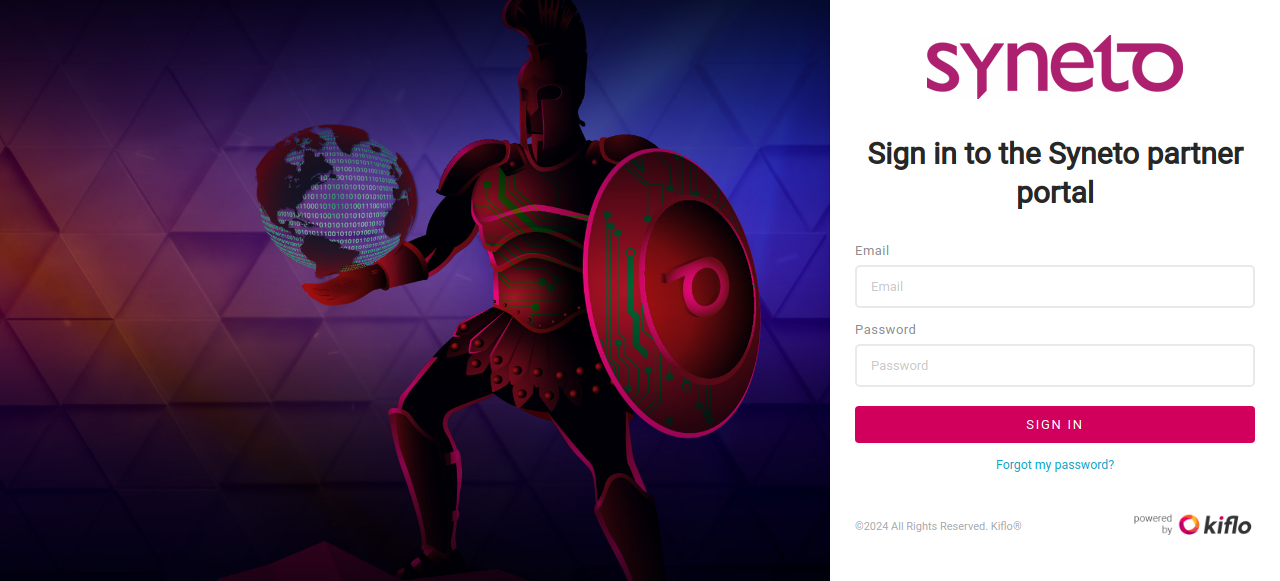
\includegraphics[width=\linewidth]{screenshots/partners.syneto.eu:443_unknown.png}
                                }
                                \vspace{0cm}
                                \captionof{figure}{Hostname: partners.syneto.eu:443 | Severity: unknown}
                                \end{center}
                                
                                
                                \begin{center}
                                \tcbox{
                                    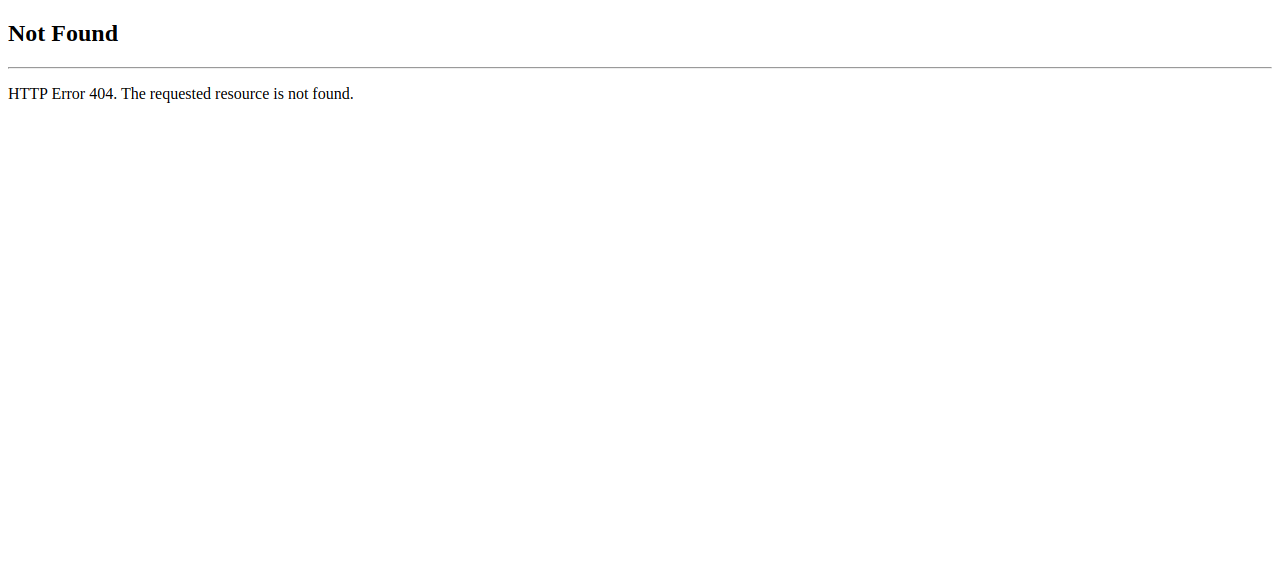
\includegraphics[width=\linewidth]{screenshots/sizer.syneto.eu_low.png}
                                }
                                \vspace{0cm}
                                \captionof{figure}{Hostname: sizer.syneto.eu | Severity: low}
                                \end{center}
                                
                                
                                \begin{center}
                                \tcbox{
                                    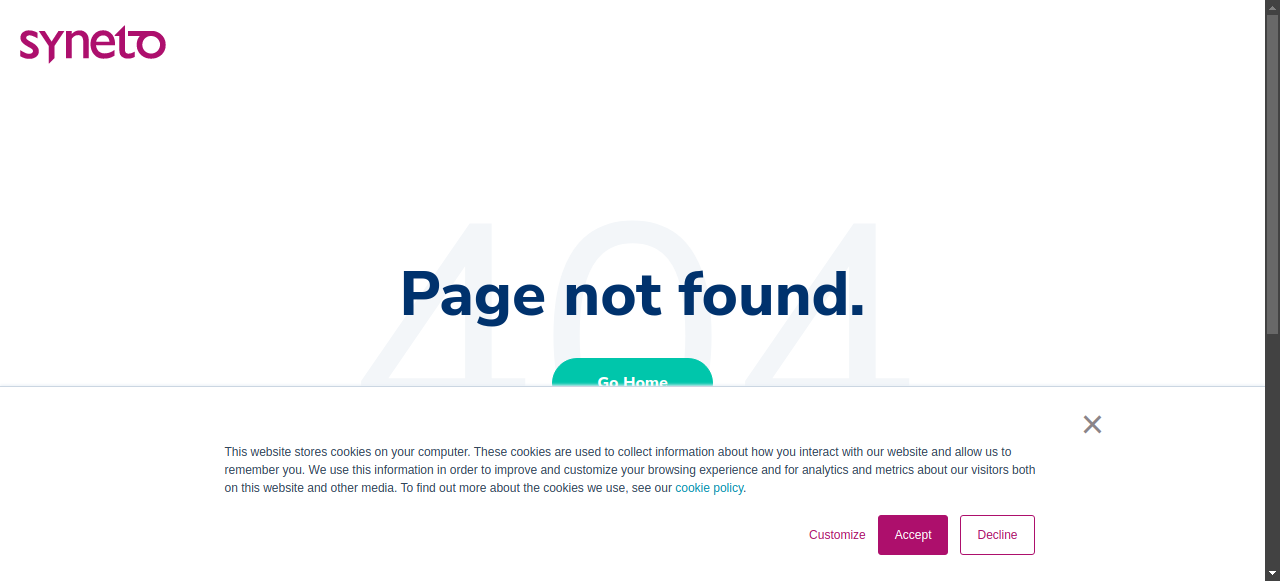
\includegraphics[width=\linewidth]{screenshots/email.syneto.eu_low.png}
                                }
                                \vspace{0cm}
                                \captionof{figure}{Hostname: email.syneto.eu | Severity: low}
                                \end{center}
                                
                                
                                \begin{center}
                                \tcbox{
                                    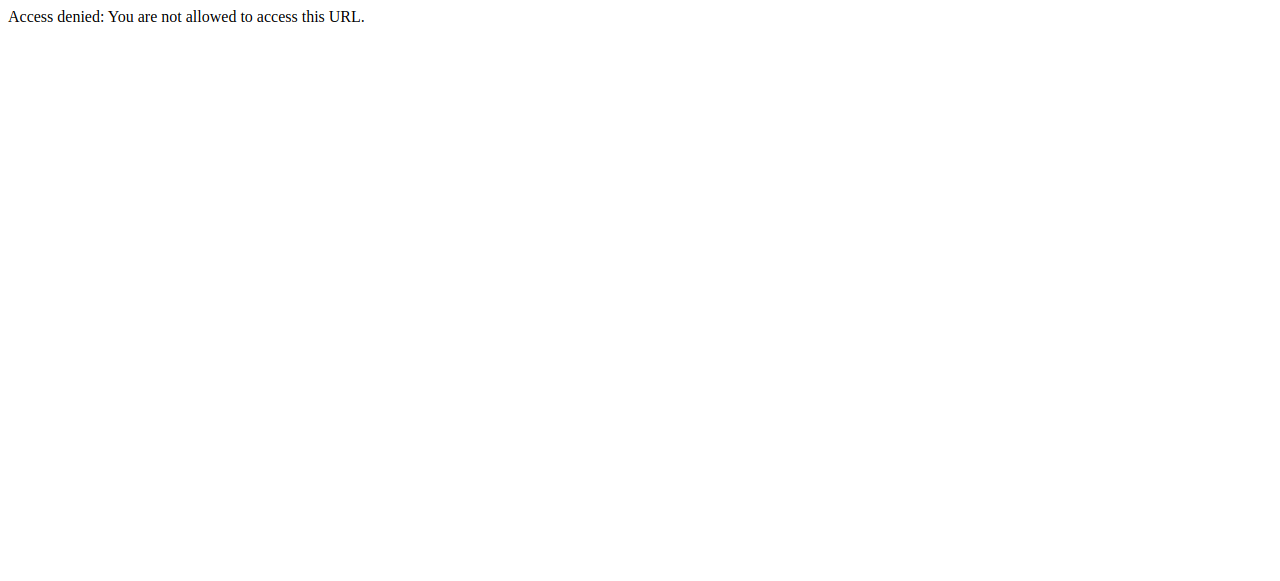
\includegraphics[width=\linewidth]{screenshots/vpn.backup.syneto.eu:5000_low.png}
                                }
                                \vspace{0cm}
                                \captionof{figure}{Hostname: vpn.backup.syneto.eu:5000 | Severity: low}
                                \end{center}
                                
                                
                                \begin{center}
                                \tcbox{
                                    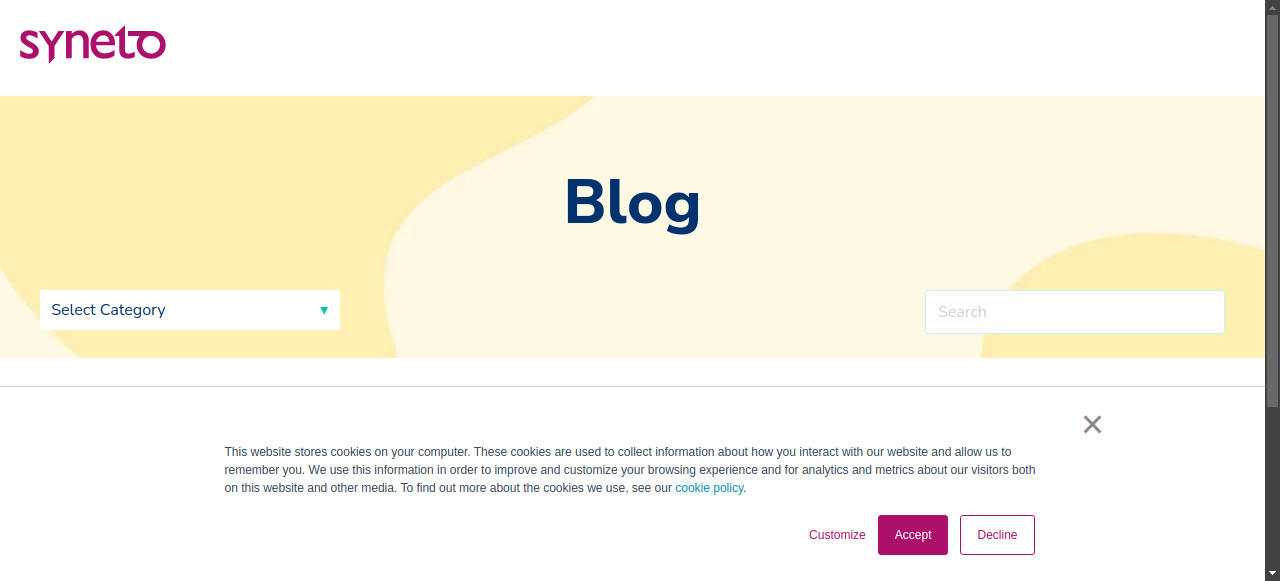
\includegraphics[width=\linewidth]{screenshots/blog.syneto.eu_low.png}
                                }
                                \vspace{0cm}
                                \captionof{figure}{Hostname: blog.syneto.eu | Severity: low}
                                \end{center}
                                
                                
                                \begin{center}
                                \tcbox{
                                    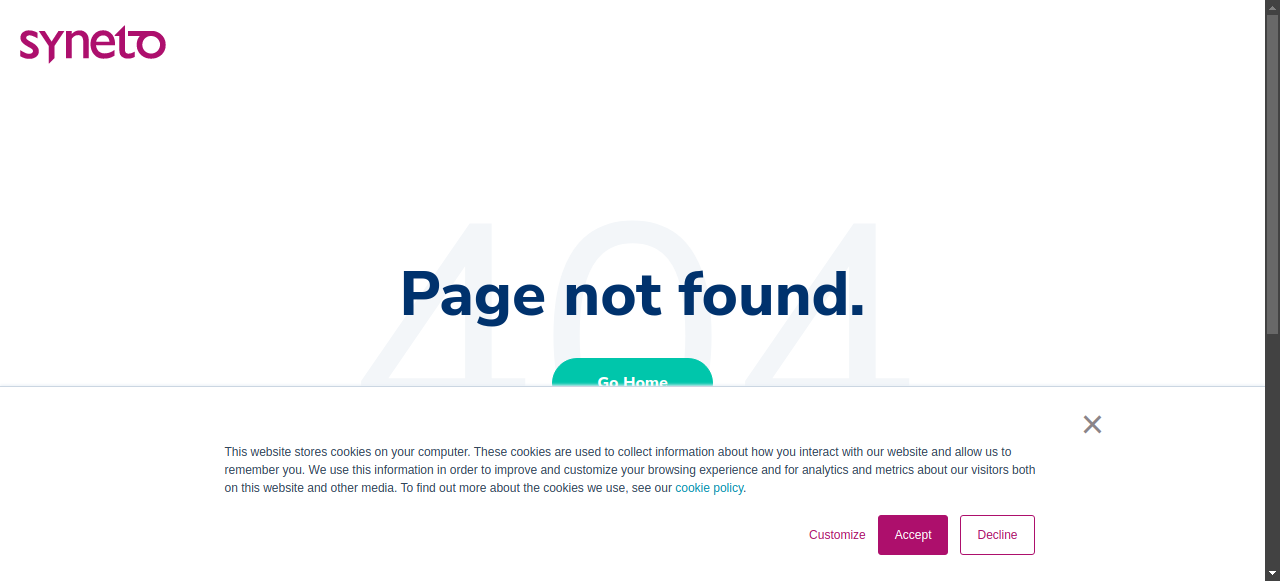
\includegraphics[width=\linewidth]{screenshots/lp.syneto.eu_low.png}
                                }
                                \vspace{0cm}
                                \captionof{figure}{Hostname: lp.syneto.eu | Severity: low}
                                \end{center}
                                
                                
                                \begin{center}
                                \tcbox{
                                    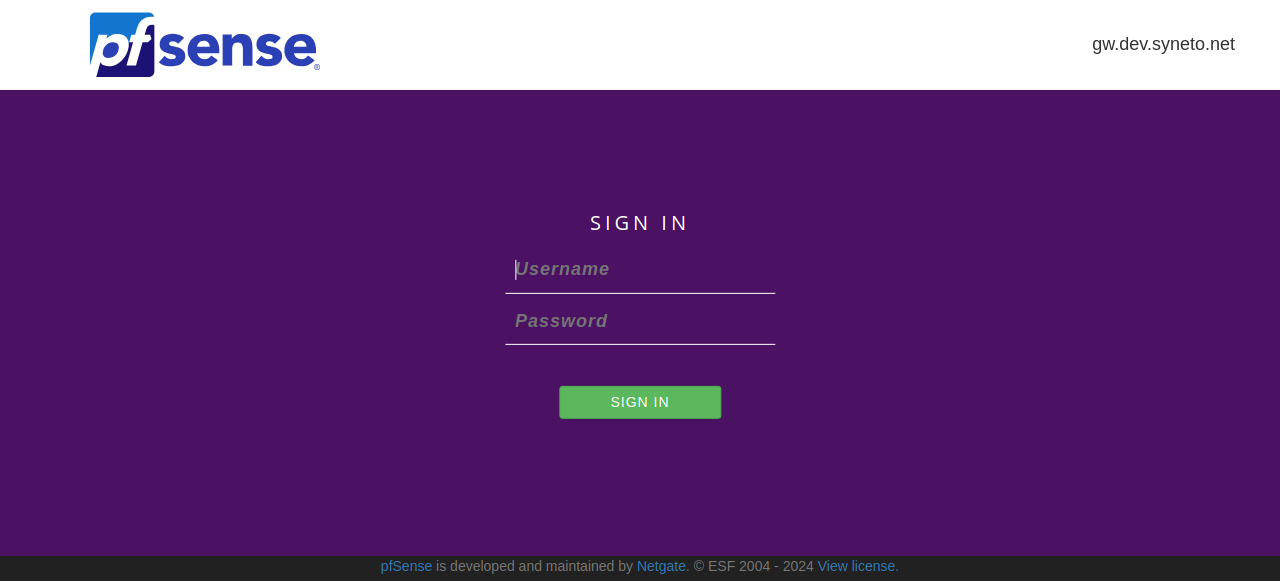
\includegraphics[width=\linewidth]{screenshots/beta-updates.syneto.eu_low.png}
                                }
                                \vspace{0cm}
                                \captionof{figure}{Hostname: beta-updates.syneto.eu | Severity: low}
                                \end{center}
                                
                                
                                \begin{center}
                                \tcbox{
                                    
\includegraphics[width=\linewidth]{screenshots/minio.syneto.eu:9000_low.png}
                                }
                                \vspace{0cm}
                                \captionof{figure}{Hostname: minio.syneto.eu:9000 | Severity: low}
                                \end{center}
                                
                                
                                \begin{center}
                                \tcbox{
                                    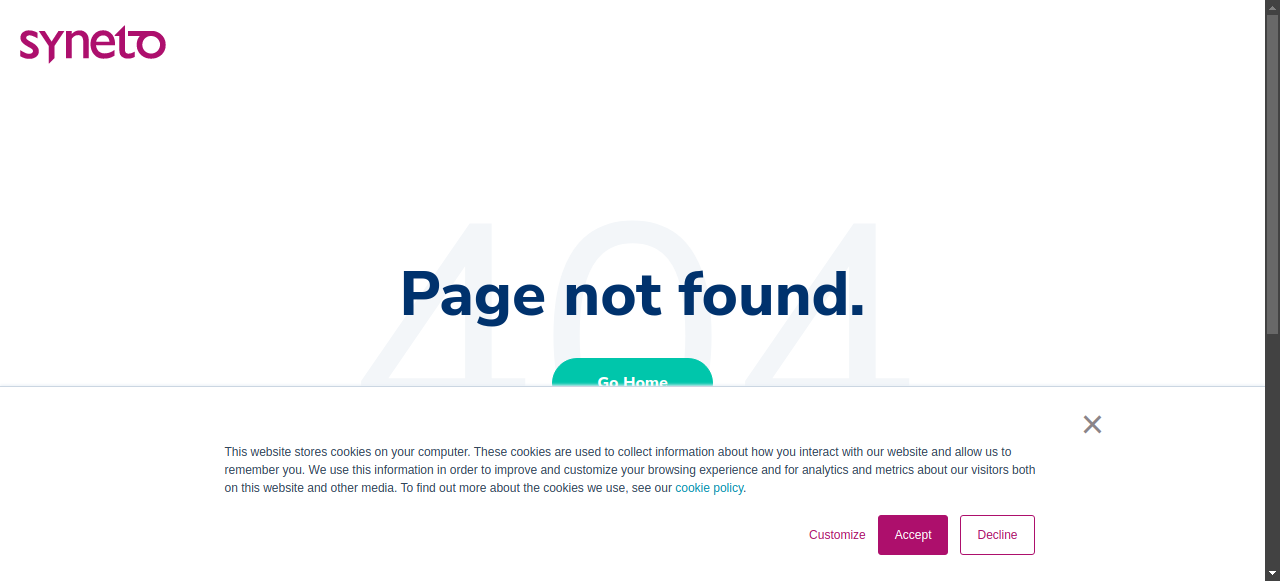
\includegraphics[width=\linewidth]{screenshots/kb.syneto.eu_low.png}
                                }
                                \vspace{0cm}
                                \captionof{figure}{Hostname: kb.syneto.eu | Severity: low}
                                \end{center}
                                
                                
                                \begin{center}
                                \tcbox{
                                    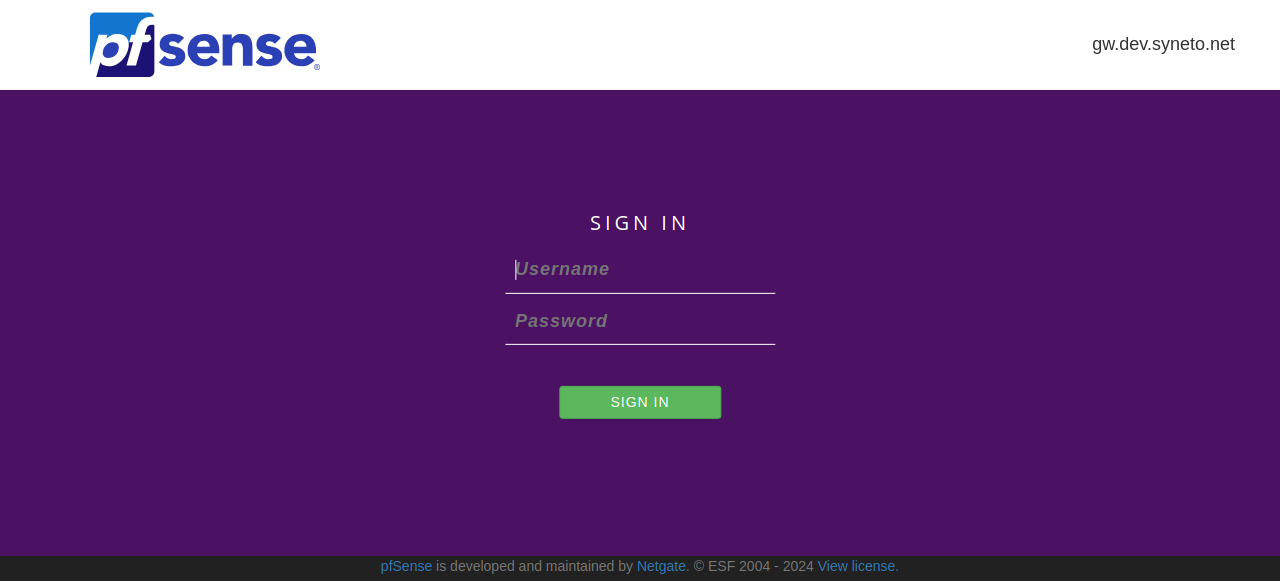
\includegraphics[width=\linewidth]{screenshots/support-data.syneto.eu_low.png}
                                }
                                \vspace{0cm}
                                \captionof{figure}{Hostname: support-data.syneto.eu | Severity: low}
                                \end{center}
                                
                                
                                \begin{center}
                                \tcbox{
                                    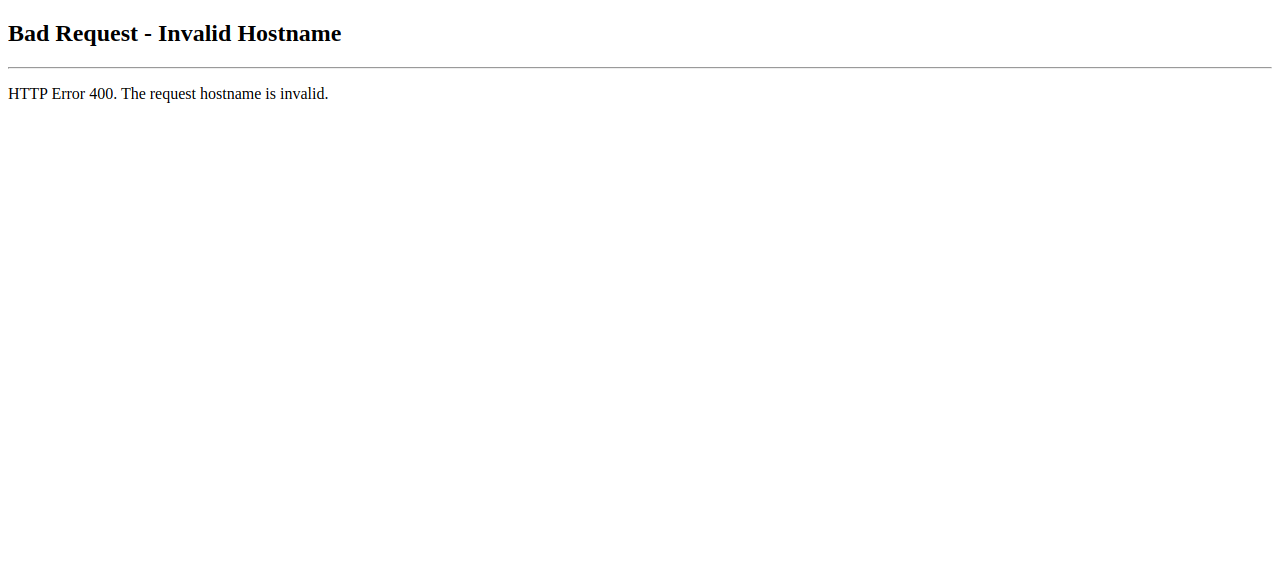
\includegraphics[width=\linewidth]{screenshots/sizer.syneto.eu:50002_low.png}
                                }
                                \vspace{0cm}
                                \captionof{figure}{Hostname: sizer.syneto.eu:50002 | Severity: low}
                                \end{center}
                                
                                